\documentclass[11pt]{article}

\usepackage{ulem}
\usepackage{tikz}
\usepackage{xurl}
\usepackage{float}
\usepackage{amsmath}
\usepackage{booktabs}
\usepackage{graphicx}
\usepackage{listings}
\usepackage[T5]{fontenc}
\usepackage{indentfirst}
\usepackage[utf8]{inputenc}
\usepackage[margin=1in]{geometry}
\usetikzlibrary{arrows.meta, positioning}

\begin{document}

\begin{center}

{\Large \textbf{UNIVERSITY OF SCIENCE AND TECHNOLOGY OF HANOI}}\\
\vspace{0.3cm}
----------------------o0o----------------------\\

\vspace{4cm}

{\large
\centerline{2540027 - Nguyễn Xuân Vinh}
}

\vspace{4cm}

{\Huge \textbf{BC3.04a Advanced Programming for HPC}}\\
\vspace{0.5cm}
Lecturer: Dr. Trần Giang Sơn

\vspace{4cm}

{\Large \textbf{REPORT LABWORK 10}}\\

\vspace{0.5cm}

{\large
Subjects: Fine-art transformation
}

\vspace{4cm}
\today
\end{center}

\newpage

\newpage

\tableofcontents

\newpage

\section{Introduction}

The purpose of the labwork 10 is to implement the Kuwahara filter for
fine-art image transformation using CUDA. The Kuwahara filter is a
non-linear image filter that can reduce noise while preserving edges.
It can also produce an oil-painting-like visual effect.

Two CUDA implementations are considered:

\begin{itemize}
    \item Kuwahara filtering using global memory.
    \item Kuwahara filtering using shared memory.
\end{itemize}

A CPU implementation is used as the baseline. Different two-dimensional
CUDA block sizes are also tested to evaluate their effect on execution
time.

The input image used in this experiment is \texttt{/content/img.jpg}.

\section{Kuwahara Filter}

For each output pixel, the Kuwahara filter considers four neighboring
windows. In this experiment, the parameter is set to

\[
\omega = 3.
\]

Therefore, each window has size

\[
(\omega+1)\times(\omega+1)
=
4\times4.
\]

The four windows are defined around the current pixel as

\[
W_1: x\in[i-\omega,i],\quad y\in[j-\omega,j],
\]

\[
W_2: x\in[i,i+\omega],\quad y\in[j-\omega,j],
\]

\[
W_3: x\in[i-\omega,i],\quad y\in[j,j+\omega],
\]

\[
W_4: x\in[i,i+\omega],\quad y\in[j,j+\omega].
\]

For each window, the mean and standard deviation of the brightness
are calculated. The window with the smallest standard deviation is
selected. The mean RGB value of that window is then assigned to the
corresponding output pixel.

\section{Implementation}

\subsection{RGB to HSV}

The Kuwahara filter uses the brightness component of the HSV color
space to calculate the standard deviation. Therefore, the input RGB
image is first converted to HSV.

Only the $V$ component is required by the filter. The $V$ component is

\[
V = \max(R,G,B).
\]

Thus, the implementation stores the $V$ channel instead of storing
unnecessary $H$ and $S$ components.

The RGB image and the corresponding $V$ channel are then provided to
the CPU and CUDA implementations.

\subsection{CPU Implementation}

The CPU implementation processes every pixel sequentially. For each
pixel, the four Kuwahara windows are examined.

For each window, the implementation calculates

\[
\mu_V = \frac{1}{N}\sum_{p\in W} V(p)
\]

and

\[
\sigma =
\sqrt{
\frac{1}{N}\sum_{p\in W}V(p)^2
-
\mu_V^2
}.
\]

The window with the lowest standard deviation is selected. The average
RGB values of this window are used as the output color.

The CPU implementation is used as the baseline for calculating CUDA
speedup.

\subsection{CUDA Implementation Without Shared Memory}

The first CUDA implementation assigns one CUDA thread to each output
pixel.

Each thread reads the required RGB and $V$ values directly from global
memory. It then calculates the statistics of the four windows and
selects the window with the lowest standard deviation.

This implementation is straightforward, but neighboring threads may
access overlapping regions of the input image. Consequently, the same
input data can be read from global memory multiple times.

\subsection{CUDA Implementation With Shared Memory}

The second CUDA implementation uses shared memory to reduce repeated
global-memory accesses.

Before processing a pixel, the threads in a CUDA block cooperatively
load the required image region into shared memory. A halo around the
block is also loaded because the Kuwahara windows extend beyond the
center pixel.

After the data is loaded, the threads synchronize using

\begin{verbatim}
cuda.syncthreads()
\end{verbatim}

The four Kuwahara windows are then calculated using the shared-memory
data rather than repeatedly reading the input image from global memory.

This allows neighboring threads to reuse image data that has already
been loaded into the shared-memory tile.

\section{CUDA Block Size Experiment}

Several two-dimensional CUDA block sizes were tested:

\begin{itemize}
    \item $4\times4$
    \item $8\times8$
    \item $16\times16$
    \item $32\times8$
    \item $32\times16$
    \item $32\times32$
\end{itemize}

The execution time was measured after CUDA kernel compilation and
warm-up. The benchmark measures the execution time of the Kuwahara
kernel itself.

\section{Results}

\subsection{Execution Time and Speedup}

The CPU execution time measured in the experiment was

\[
T_{\mathrm{CPU}} = 1.140110\text{ s}.
\]

The fastest global-memory CUDA configuration was the $32\times16$
block size:

\[
T_{\mathrm{global}} = 0.016386\text{ s}.
\]

Therefore, the speedup over the CPU implementation was

\[
S_{\mathrm{global}}
=
\frac{T_{\mathrm{CPU}}}{T_{\mathrm{global}}}
=
\frac{1.140110}{0.016386}
\approx 69.58.
\]

Thus, the global-memory CUDA implementation achieved a measured
speedup of approximately $69.58\times$ compared with the CPU
implementation.

The fastest shared-memory CUDA configuration was the $16\times16$
block size:

\[
T_{\mathrm{shared}} = 0.016296\text{ s}.
\]

Its speedup over the CPU implementation was

\[
S_{\mathrm{shared}}
=
\frac{T_{\mathrm{CPU}}}{T_{\mathrm{shared}}}
=
\frac{1.140110}{0.016296}
\approx 69.96.
\]

The measured speedup of the shared-memory implementation over the
global-memory implementation was

\[
S_{\mathrm{shared/global}}
=
\frac{T_{\mathrm{global}}}{T_{\mathrm{shared}}}
=
\frac{0.016386}{0.016296}
\approx 1.01.
\]

The main measured results are summarized in Table~\ref{tab:summary}.

\begin{table}[H]
\centering
\caption{Main performance results}
\label{tab:summary}
\begin{tabular}{lcc}
\toprule
Implementation & Execution Time (s) & Speedup \\
\midrule
CPU & 1.140110 & $1.00\times$ \\
CUDA Global ($32\times16$) & 0.016386 & $69.58\times$ \\
CUDA Shared ($16\times16$) & 0.016296 & $69.96\times$ \\
\bottomrule
\end{tabular}
\end{table}

The shared-memory implementation was approximately $1.01\times$ faster
than the fastest global-memory configuration in this experiment.

\subsection{Correctness}

The CUDA results were compared with the CPU output.

For the fastest global-memory configuration, the maximum pixel
difference compared with the CPU result was

\[
\text{Max Difference}_{global}=0.
\]

For the fastest shared-memory configuration, the maximum difference
was also

\[
\text{Max Difference}_{shared}=0.
\]

Therefore, both CUDA implementations produced the same output as the
CPU implementation for the tested image.

\section{Performance Considerations}

The main optimization in the shared-memory implementation is data
reuse. A Kuwahara window contains multiple neighboring pixels, and
neighboring CUDA threads require many of the same input pixels. With
global memory, these values may be loaded repeatedly.

The shared-memory implementation loads a larger tile containing the
block region and its surrounding halo. The loaded values can then be
reused by all threads in the block.

The global-memory loading pattern is arranged according to the
two-dimensional image layout, allowing neighboring threads to access
neighboring image locations during tile loading. The shared-memory
implementation subsequently performs the window calculations from the
local shared-memory tile.

No additional shared-memory padding was introduced specifically to
eliminate bank conflicts. The main optimization evaluated in the
labwork 10 is therefore the reduction of repeated global-memory accesses
through shared-memory reuse.

The measured improvement between the fastest global and shared
implementations was relatively small:

\[
1.01\times.
\]

This indicates that, for the tested image, filter size, and CUDA
configuration, global-memory access was already highly effective and
the additional shared-memory optimization provided only a small
measured benefit.

\section{Result Images}

The original image and the Kuwahara filter results are shown below.

\begin{figure}[H]
    \centering
    
\includegraphics[width=0.8\textwidth]{original.png}
    \caption{Original input image}
    \label{fig:original}
\end{figure}

\begin{figure}[H]
    \centering
    
\includegraphics[width=0.8\textwidth]{cpu_kuwahara.png}
    \caption{CPU Kuwahara result}
    \label{fig:cpu}
\end{figure}

\begin{figure}[H]
    \centering
    
\includegraphics[width=0.8\textwidth]{gpu_global_kuwahara.png}
    \caption{CUDA Kuwahara using global memory}
    \label{fig:global}
\end{figure}

\begin{figure}[H]
    \centering
    
\includegraphics[width=0.8\textwidth]{gpu_shared_kuwahara.png}
    \caption{CUDA Kuwahara using shared memory}
    \label{fig:shared}
\end{figure}

The comparison of the CPU, global-memory CUDA, and shared-memory CUDA
outputs is shown in Figure~\ref{fig:comparison}.

\begin{figure}[H]
    \centering
    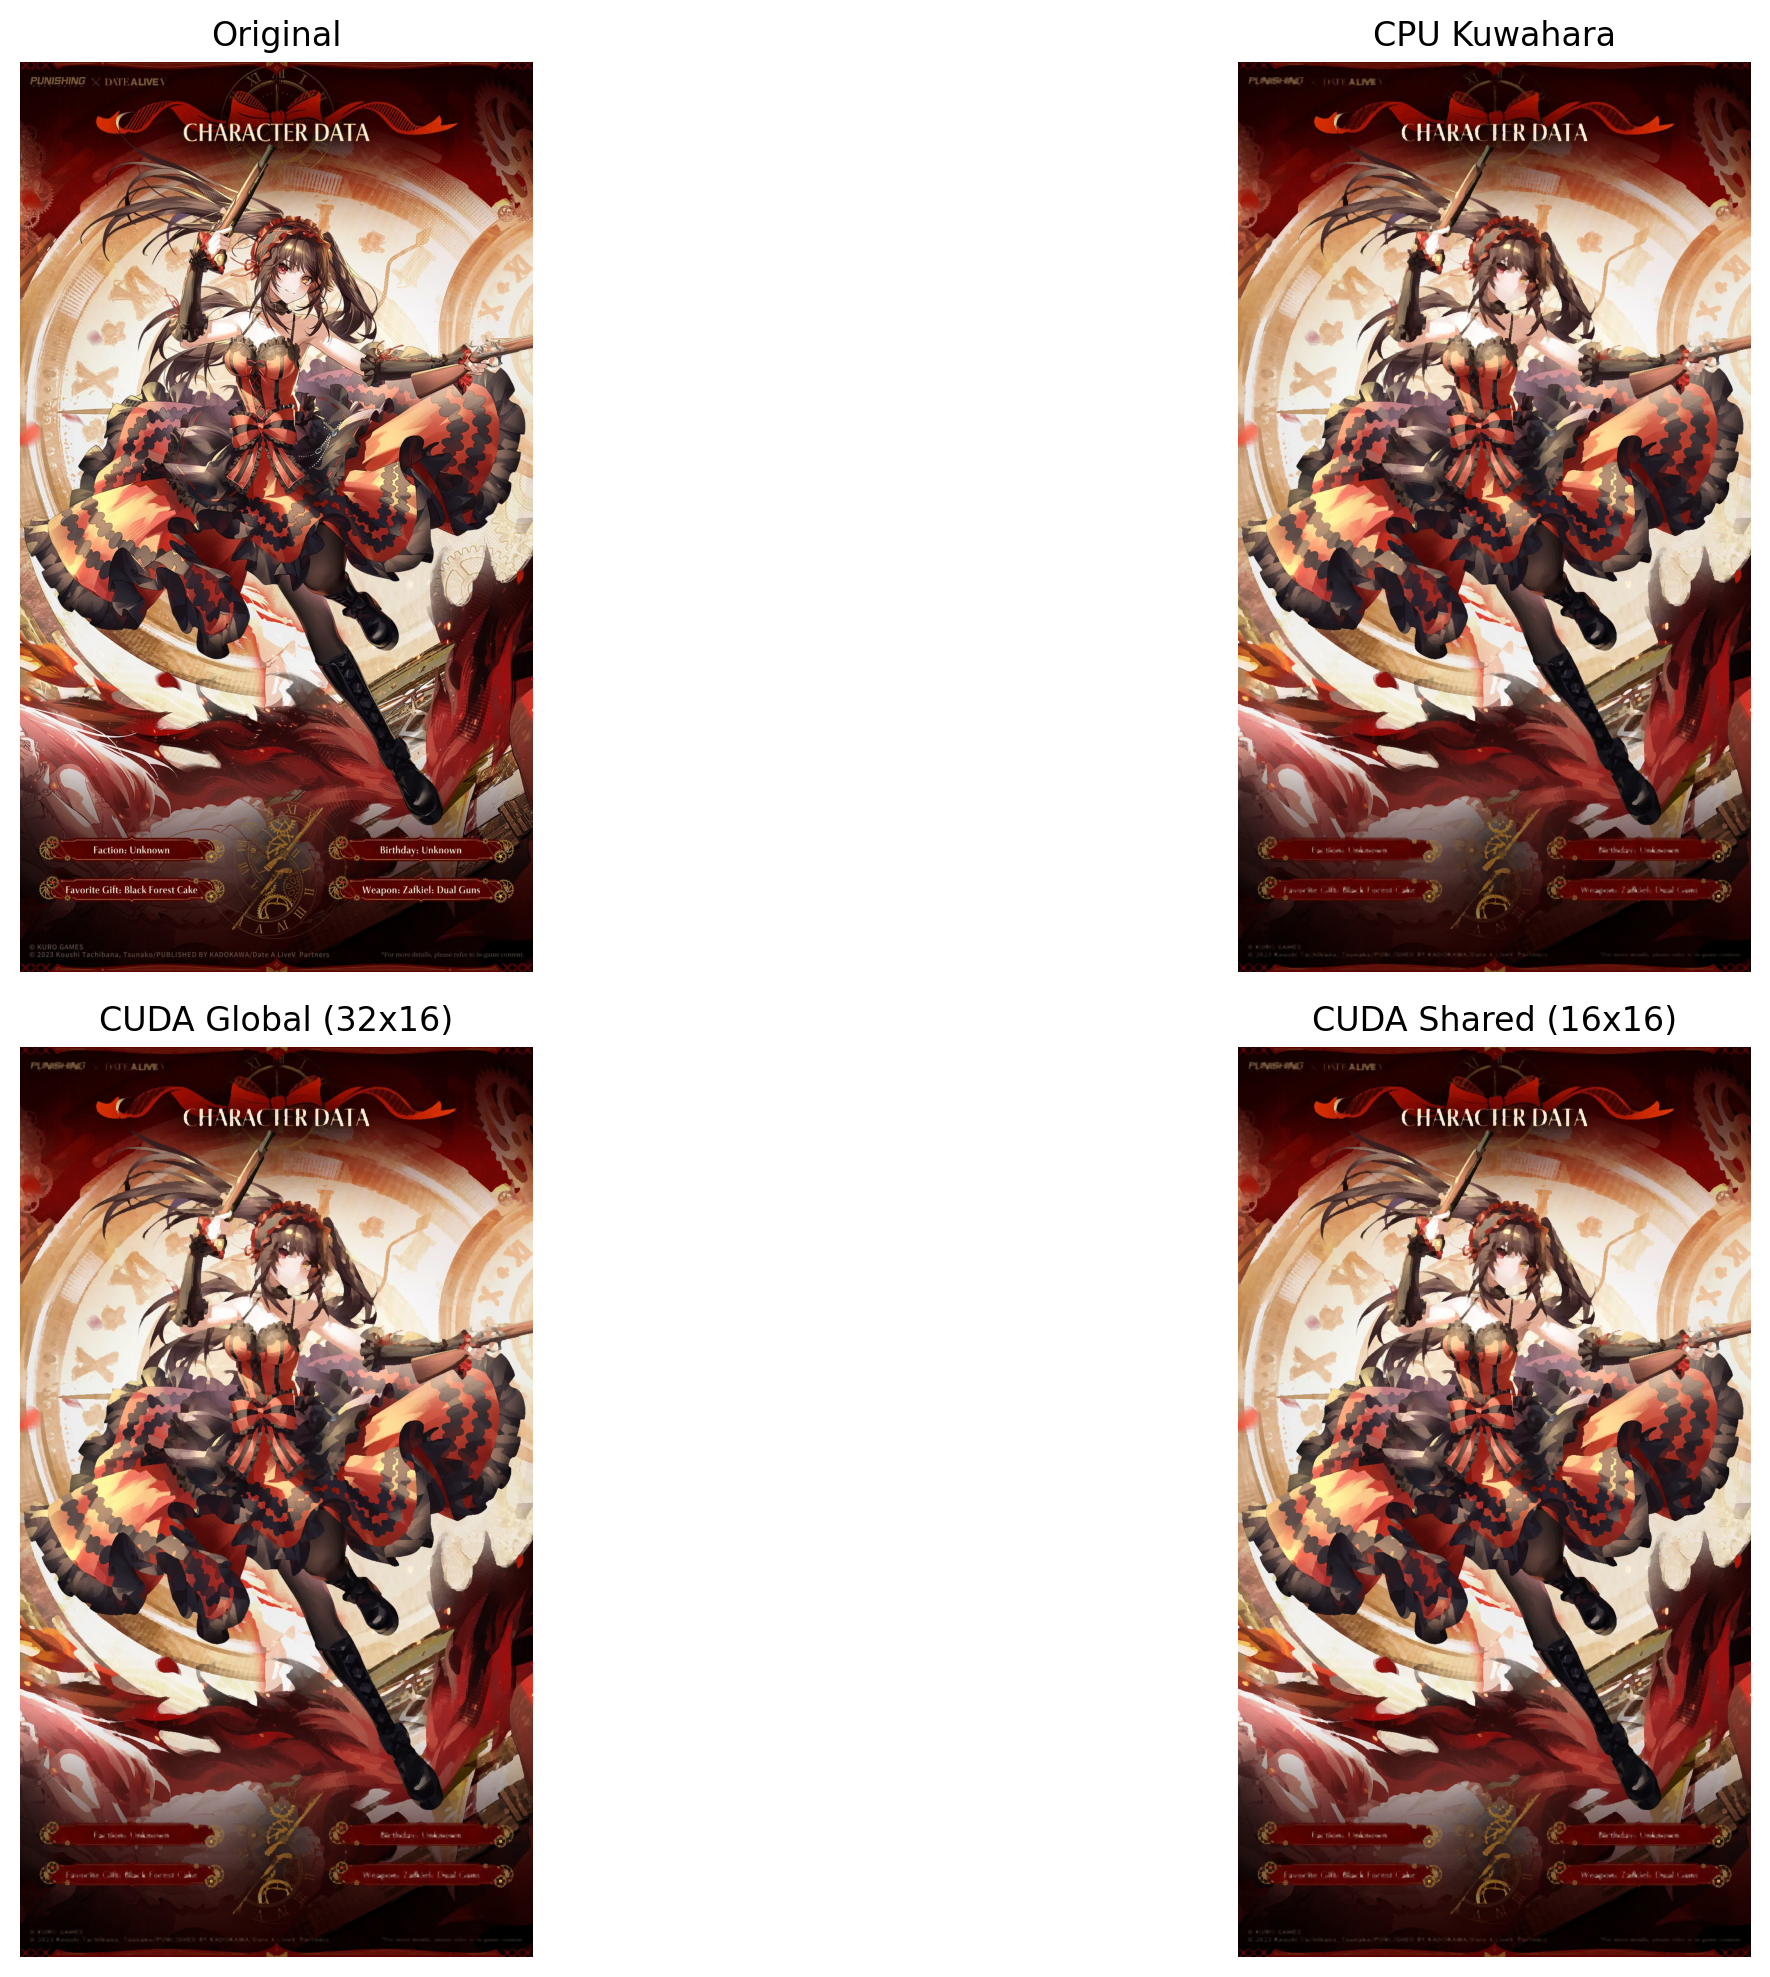
\includegraphics[width=\textwidth]{comparison.png}
    \caption{Comparison of CPU and CUDA Kuwahara results}
    \label{fig:comparison}
\end{figure}

\section{Conclusion}

In the 10 labwork, the Kuwahara filter was implemented using a CPU
version and two CUDA versions. The CUDA implementations use the same
four-window Kuwahara algorithm and the HSV $V$ channel to calculate
the brightness standard deviation.

The CPU implementation required $1.140110$ seconds. The fastest
global-memory CUDA implementation used a $32\times16$ block and
required $0.016386$ seconds, giving a measured speedup of
$69.58\times$.

The fastest shared-memory CUDA implementation used a $16\times16$
block and required $0.016296$ seconds, giving a measured speedup of
$69.96\times$ over the CPU implementation. Compared with the fastest
global-memory implementation, the shared-memory version achieved a
$1.01\times$ speedup.

Both CUDA implementations produced results with a maximum difference
of zero compared with the CPU output. Therefore, the GPU
implementations preserved the correctness of the CPU reference while
providing a substantial reduction in execution time.

\end{document}